\documentclass[../thesis.tex]{subfiles}
\begin{document}
\chapter{Theory}\label{cap:theory}

\section{Human-Robot Interaction}
At the present there are several ways to interact with a robot. The best way to do it, generally, depends on the type of robot and on the task it has to perform. It is possible to compare two ways for a human to interact with a robot:
\begin{itemize}
    \item Using a third party device that acts as a controller like a joystick or a computer with an user interface to control the robot;
    \item Using his/her own body, in particular using hand gestures, the voice or the body position.
\end{itemize}
\subsection{Using a third party device}
The oldest ways to interact with a robot involve the use of a controller that the operator must use to tell the robot what actions perform. In this case, the controller could be a joystick or a computer program. In the last case, the study of \acrfull{HCI} must be considered. Using a third-party device to control a robot is not the easiest way, especially when the tasks to complete are intricate and the robot's movements are as complicated as the tasks.  
%Provide some examples of these kind of interactions

\subsection{Using the human body}
The other way to interact with a robot involves the use of the human body. The robot can get input signals through microphones and cameras. The operator can give input through his/her voice, in this case \acrfull{NLP} is involved, otherwise the operator can give input with hand gestures, body position or even with facial expressions.For example,~\citeauthor{paper:commanding_a_robot_with_NLP} achieved an accuracy between the $70\%$ and $80\%$ in converting raw input text into robot commands through \acrshort{NLP} techniques~\cite{paper:commanding_a_robot_with_NLP}. Better results are achieved when the full body position is exploited. For example, \citeauthor{paper:example_full_body_gesture1} exploited the body position to recognize gestures such as walking, running, bending, jumping, lying down on the floor, waving a hand, sitting on the floor, raising the right hand, getting down on the floor, and touching a knee and wrist with a generally high accuracy ($~95\%$)~\cite{paper:example_full_body_gesture1}.~\citeauthor{paper:example_full_body_gesture2} also reached similar results in~\citeyear{paper:example_full_body_gesture2} recognizing four gesture~\cite{paper:example_full_body_gesture2}. Regarding the hand gestures, the literature has some interesting experiments that exploited them to control a computer or a robot.~\citeauthor{paper:design_and_evaluate_hand_gesture} in~\citeyear{paper:design_and_evaluate_hand_gesture} designed and evaluated six hand gestures to interact with a computer. The results are outstanding with an accuracy of $97\%$~\cite{paper:design_and_evaluate_hand_gesture}. Finally, let me present the work made by~\citeauthor{paper:intuitiveness_level} to define which gestures use to interact with a robot considering the ``Intuitiveness Level''~\cite{paper:intuitiveness_level}. The proposed methodology is composed of four steps:
\begin{enumerate}
    \item \textbf{Choice of tasks}: select a set of tasks that the robot will perform.
    \item \textbf{Capture of gestural data}: an user-based approach is suggested. An intuitive gesture is one that comes from the subconscious mind. You can ask some volunteers to perform some gestures related to the task until they are out of ideas. This approach is called, by the author, ``Frustration Based Approach''.
    \item \textbf{Analysis of captured gestures}: each gesture is analyzed finding the most common and the most compatible with the task.
    \item \textbf{Choice of vocabulary} (intuitiveness table): the set of gestures is chosen. The decision is made looking at the \glsfirst{IL}.
\end{enumerate}

\section{Hand gesture recognition}
The hand gesture recognition task is a well-studied task. In the literature is possible to find the idea to use the hand gesture as a way to interact with a machine since 1987~\cite{paper:hand_gesture_interface_device}. At that time the idea was to use a glove to recognize the position and the orientation of the user's hand. They were thought to be used for different tasks like gesture recognition, an interface to a visual programming language, virtual object manipulation, and many others. Nowadays, even if a wearable device to recognize what the hands are doing is highly accurate and precise, for some tasks it is possible to reach a good level of accuracy with only a webcam. Especially, thanks to the increase of computing power, also in small devices and the improved quality of video acquisition devices, the study of computer vision and machine learning techniques to recognize hand gestures is becoming very interesting.

\subsection{Machine learning}
Recognizing a hand gesture given an image or a frame of a video is not something easily algorithmizable. For this, the idea of using a neural network to fulfill the task is a good one.

\subsubsection{Neural network}
A neural network is a collection of neurons connected together. For the biology a neuron is an entity that takes several inputs, sums them together and, if a threshold is surpassed emits an output. An artificial neuron is similar. Figure~\ref{fig:neuron} represents one of them. It takes $N$ inputs, sums them together with a bias and passes the result to an activation function. If the result is higher than a threshold then the neuron returns an output.

\begin{figure}[H]
    \centering
    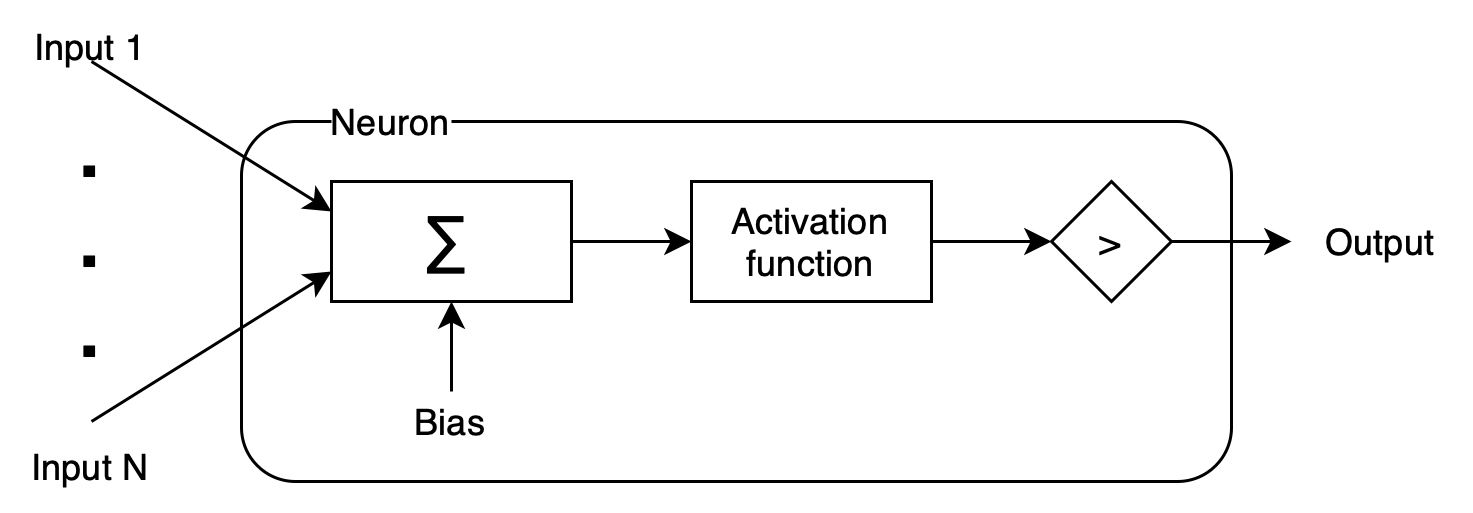
\includegraphics{thesis/images/neuron.png}
    \caption{Representation of a neuron in a neural network.}
    \label{fig:neuron}
\end{figure}

An artificial neural network is a set of neurons organized in layers. Figure~\ref{fig:neural_network_example} represents a deep neural network, deep because there is one or more hidden layer. Different kind of layers exists, the one showed in figure~\ref{fig:neural_network_example}, other than input and output, is a dense layer. In this kind of layer every output of the previous layer is received in input by each neuron of the layer considerate for the reasoning. Regarding the output layer, each neurons return a probability that the input belongs to a class. When there is only one output neuron the probability is $p$ to belong to the class an $1-p$ to not belong to the class. When there are more than one neurons, each of them return the probability to belong to a class and the highest is taken as the prediction. A prediction, to be considerated correct, must overcome a threshold value. More are the hidden layer, more the network will be accurate but, more time will take to learn.

\begin{figure}[H]
    \centering
    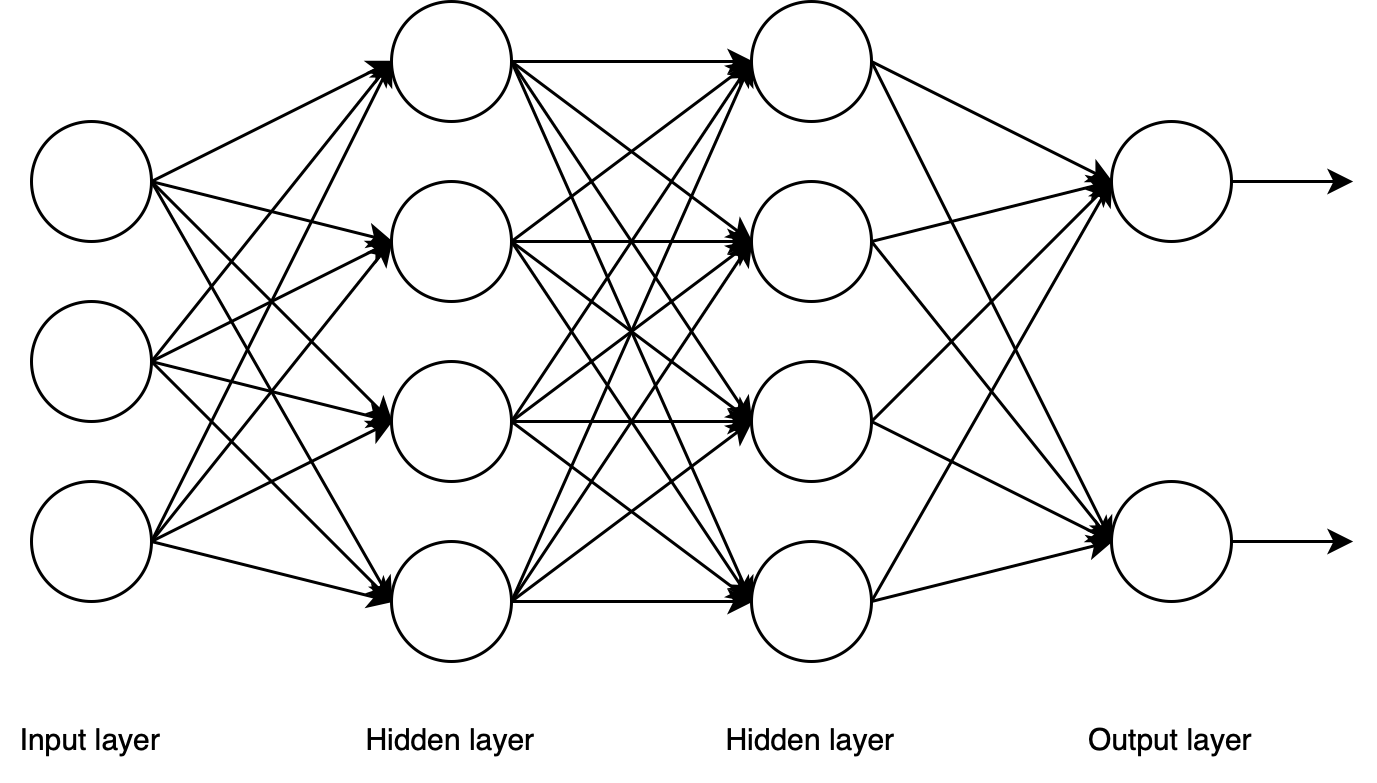
\includegraphics{thesis/images/neuralNetworkExample.png}
    \caption{An example of a deep neural network}
    \label{fig:neural_network_example}
\end{figure}

\subsubsection{Dataset}
When \acrshort{ML} is involved, the challenge is the need for big datasets on which the network can train. When image recognition is the task to fulfill, the datasets are composed of a lot of images and each one must be labeled to know what it is representing and where, inside the image, the position of the object to detect is. This kind of training is known as supervised learning which is different from the unsupervised in which the dataset has no labels and usually the task is to categorize the elements into macro-categories. Regarding the dataset dimension, I stress that, bigger is the dataset, slower is the training task. It is important find the right dimension that allows to have an acceptable accuracy level.

\subsubsection{Training}
The goal of training a neural networks is to find the best weights for each neuron's inputs. The gradient descent technique is used to achieve this goal. Data is essential to train a neural network. To correctly train and evaluate a neural network, three datasets are requested. Usually, one dataset is divided in three non-overlapping partitions in a random way. The first and the biggest part of the dataset is used to train the network. In detail, it is used for adjust the weights of inputs. Then, another part of the dataset is picked as validation during the training process and the last part is taken to evaluate the trained model at the end.

\subsubsection{Evaluation}
To evaluate an \acrshort{ML} model is necessary to collect some data during the training process. The metrics to keep track of are:
\begin{itemize}
    \item \textbf{loss function}: what the network aims to minimize. Generally, it represents the prediction error with respect to the ground truth.
    \item \textbf{accuracy}: is the ratio between the number of correct predictions, and the total number of predictions made.
        \begin{equation}
                Accuracy = \frac{Number\, of\, right\, predictions}{Number\, of\, predictions}
        \end{equation}
    \item \textbf{time}: the time spent on training the network. It depends on the dataset size and the complexity of the network. Specifically, a bigger dataset will require more time but will give better results as well as a more complex network.
\end{itemize}
The best neural network is the one that guarantees the best trade-off between these metrics.

\subsubsection{State of the art}
At present, there are several ways to achieve good results in the hand gesture recognition task with the help of neural networks. The results presented in~\citeauthor{paper:survey_on_vision_based_hand_gesture_recognition}~\cite{paper:survey_on_vision_based_hand_gesture_recognition} shows that with a \acrfull{CNN} is possible to achieve accuracy higher than the $90\%$. \acrshortpl{CNN} are classifier-based systems that can process input images as structured arrays of data and identify patterns between them. To date, there are two main types of object detection algorithms in the field of deep learning:
\begin{itemize}
    \item \textbf{Classification-based algorithms}: firstly, they select a group of \acrfullpl{ROI} in the images where the chances that an object is present are high; secondly, they apply \acrshort{CNN} techniques to these selected regions to detect the presence of an object. A problem associated with these types of algorithms is that they need to execute a detector in each \acrshort{ROI}, and this makes the process of object detection very slow and highly expensive in terms of computation.
    \item \textbf{Regression-based algorithms}: these types of algorithms are faster than the above algorithms, in that there is no selection of the \acrshort{ROI} so that the bounding boxes and the labels are predicted for the whole image at once; they can identify and classify objects within the image at once. Beyond the higher speed, a key point is that the predictions are informed by the global context in the image, thus they generally lead to higher accuracies.
\end{itemize}
One of the most famous regression-based algorithms is \glsfirst{YOLO}, but it is not the only possible solution to perform this kind of task. Another technique, that gives promising results is the combination of the MediaPipe hand tracker, which section~\ref{sec:mediapipe} describes, and a feed-forward neural network to recognize the gesture.\\
All these kind of solutions suit well in the case of static hand gestures. As \citeauthor{site:hand_gesture_base_repo} shows in his repository\cite{site:hand_gesture_base_repo}, working with a history of landmarks is possible. For this kind of task, a \glsfirst{LSTM} neural network is a good starting point. This kind of network tries to add the knowledge of past events to the computation, to do so there are loops inside them allowing information to persist~\cite{site:understanding_lstm_networks}.

\end{document}
